\chapter{Distribuzione gaussiana}
In questo capitolo vengono fornite le proprietà di base delle distribuzioni gaussiane, con particolare attenzione nei riguardi della \textbf{distribuzione gaussiana multivariata}. Come suggerisce il nome, i \textbf{processi gaussiani} si basano infatti su queste distribuzioni multivariate, sfruttando le proprietà che verranno mostrate nel corso del capitolo.\\
Le fonti usate per la stesura del capitolo sono \cite{gut_intermediate_2009}, \cite{wilkinson_introduction_2020}, \cite{murphy_probabilistic_2022}.


\begin{textblock*}{0.64\textwidth}(3.5cm+0.36\textwidth,18.5cm)
\epigraph{At a purely formal level, one could call probability theory the study of measure spaces with total measure one, but that would be like calling number theory the study of strings of digits which terminate.}{Terence Tao}
\end{textblock*}

\newpage

%%%%%%%%%%%%%%%%%%%%%%%%%%%%%%%%%%%
%%%%%% GAUSSIANA UNIVARIATA
%%%%%%%%%%%%%%%%%%%%%%%%%%%%%%%%%%%


\section{Distribuzione gaussiana univariata}
\begin{defi}[Distribuzione gaussiana univariata]
La \textbf{distribuzione gaussiana univariata} è una distribuzione di probabilità continua. \\
Data $Y\sim \mathcal{N}(\mu, \sigma^2)$, la sua funzione di densità di probabilità si esprime come:
\[f_Y(y) = \frac{1}{\sqrt{2\pi \sigma^2}} \text{exp}\bigg\{-\frac{1}{2}\frac{(y-\mu)^2}{\sigma^2}\bigg\}.\]
\end{defi}


%%%%%%%%%%%%%%%%%%%%%%%%%%%%%%%%%%%
%%%%%% IMMAGINI GAUSSIANA
%%%%%%%%%%%%%%%%%%%%%%%%%%%%%%%%%%%
\begin{figure}[h]
\centering
\begin{subfigure}{.5\textwidth}
  \centering
  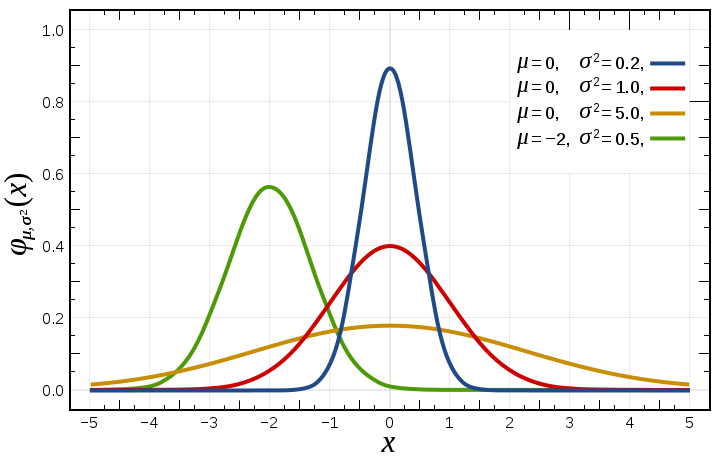
\includegraphics[width=\linewidth]{images/Gaussiane/PDFNormalDistribution.png}
  \caption{Densità di probabilità}
  \label{fig:sub1}
\end{subfigure}%
\begin{subfigure}{.5\textwidth}
  \centering
  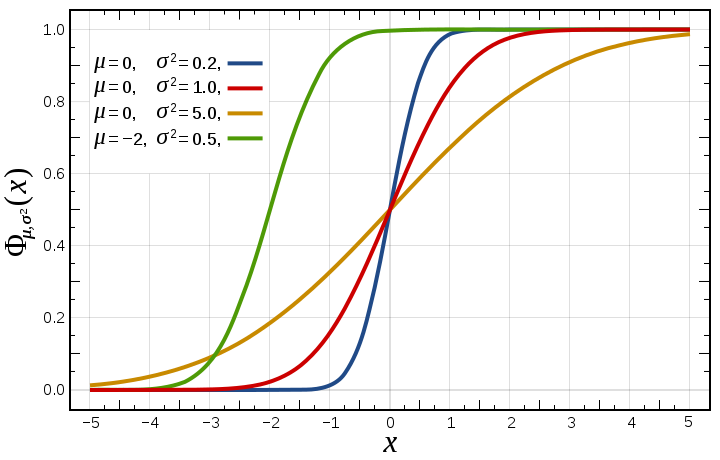
\includegraphics[width=\linewidth]{images/Gaussiane/CDFNormalDistribution.png}
  \caption{Funzione di ripartizione}
  \label{fig:sub2}
\end{subfigure}
\caption{Funzione di ripartizione e densità di probabilità di una distribuzione normale standard \cite{wikiNormalDistribution}.}
\label{fig:gaussian}
\end{figure}



\begin{oss} \label{normal decomposition}
Data $Z\sim \mathcal{N}(0,1)$ segue:  $Y=\mu + \sigma Z\sim \mathcal{N}(\mu,\sigma^2)$.
\end{oss}

\begin{oss}
Informalmente parlando, la distribuzione gaussiana è "conveniente" matematicamente per via delle sue proprietà:
\begin{itemize}
    \item la distribuzione normale ha due parametri di facile interpretazione: la media e la varianza;
    \item la distribuzione normale è chiusa per operazioni lineari;
    \item la distribuzione normale è chiusa per marginalizzazione e condizionamento (si veda la proposizione \ref{marginale-condizionata});
    \item a parità di media e varianza, la distribuzione normale ha massima entropia;
    \item dal \textbf{teorema del limite centrale}, la distribuzione normale è il limite di una somma di variabili aleatorie; occorre cioè naturalmente;
    \item la distribuzione normale ha una forma matematica semplice che ne facilita l'implementazione.
\end{itemize}
\end{oss}


\newpage


%%%%%%%%%%%%%%%%%%%%%%%%%%%%%%%%%%%
%%%%%% GAUSSIANA MULTIVARIATA
%%%%%%%%%%%%%%%%%%%%%%%%%%%%%%%%%%%
\section{Distribuzione gaussiana multivariata}


La distribuzione gaussiana multivariata è una generalizzazione della distribuzione normale (univariata).



\begin{defi}[Distribuzione gaussiana multivariata] Un vettore $n$-dimensionale $\mathbf{X}$ di variabili aleatorie è detto normale (\textbf{multivariato normale}) se e solo se $\forall \mathbf{a}\in \mathbb{R}^n$ la variabile aleatoria $\mathbf{a}^\text{T}\mathbf{X}$ è una distribuzione normale.  
La densità\footnote{Nel caso generalizzato non è possibile definire la densità della distribuzione gaussiana multivariata. Come verrà mostrato in seguito, nei processi gaussiani la densità non è importante quanto la matrice di covarianza e il vettore media.} di una \textbf{distribuzione gaussiana multivariata} si esprime come
\[f_{\mathbf{X}}(\mathbf{x})=\frac{1}{(2\pi)^{\sfrac{n}{2}}  \text{det}(\bm{\Sigma})^{\sfrac{1}{2}}} \text{ exp}\left[-\frac{1}{2}(\bm{x}-\bm{\mu})^\text{T}\bm{\Sigma}^{-1}(\bm{x}-\bm{\mu})\right]
\]\end{defi}
dove $\bm{\mu}=\mathbb{E}[\bm{X}]\in \mathbb{R}^n$ è il \textit{vettore media}, $\bm{\Sigma}=\text{Cov}[\bm{X}]$ è una matrice $n\times n$ chiamata \textit{matrice di covarianza}, definita come segue:
\[\begin{split}
\text{Cov}[\bm{X}] &= \mathbb{E}\left[(\bm{X}-\mathbb{E}[\bm{X}])(\bm{X}-\mathbb{E}[\bm{X}])^\text{T} \right]\\
 & = \begin{pmatrix}
    \mathbb{V}[X_1] & \text{Cov}[X_1,X_2] & \dots & \text{Cov}[X_1,X_n]\\
    \text{Cov}[X_2,X_1] & \mathbb{V}[X_2] & \dots & \text{Cov}[X_2,X_n]\\
    \vdots & \vdots & \ddots & \vdots\\
    \text{Cov}[X_n,X_1] & \text{Cov}[X_n,X_2] & \dots & \mathbb{V}[X_n]
    \end{pmatrix}
\end{split}
\]
dove:
\[ \text{Cov}[X_i,X_j]=\mathbb{E}[(X_i-\mathbb{E}[X_i])(X_j-\mathbb{E}[X_j])] = \mathbb{E}[X_iX_j]-\mathbb{E}[X_i]\mathbb{E}[X_j]  \]
\[ \mathbb{V}[X_i]=\text{Cov}[X_i, X_i]. \]


\begin{oss}\label{ossGaussianaMultivariata}
La matrice di covarianza è simmetrica e semidefinita positiva, cioè: $\forall \mathbf{a}\in \mathbb{R}^n$ si ha $\mathbf{a}^\text{T}\mathbf{\Sigma} \mathbf{a}\geq 0$.
\end{oss}


%%%%%%%%%%%%%%%%%%%%%%%%%%%%%%%%%%%
%%%%%% COROLLARIO DEFINIZIONE
%%%%%%%%%%%%%%%%%%%%%%%%%%%%%%%%%%%
\begin{cor}
Dato $\mathbf{X}$ un vettore multivariato normale, dalla definizione di distribuzione gaussiana multivariata seguono immediatamente:
\begin{enumerate}
    \item ogni componente di $\mathbf{X}$ è una variabile aleatoria gaussiana;
    \item $\sum_{i=1}^{n} a_iX_i$ è una variabile aleatoria gaussiana $\forall a_i\in \mathbb{R}$;
    \item se le componenti di $\mathbf{X}$ sono variabili aleatorie gaussiane indipendenti, allora $\mathbf{X}$ è un vettore multivariato normale.
\end{enumerate}
\end{cor}

\begin{oss}
Il terzo punto del corollario precedente non vale se le componenti non sono indipendenti. Per esempio: $X\sim \mathcal{N}(0,1)$, $Z\indep X$,  $\mathbb{P}(Z=1)=\mathbb{P}(Z=-1)=\sfrac{1}{2}$. Si vede facilmente che $Y=ZX$ non è indipendente da $X$ e $\begin{pmatrix}
X\\
Y
\end{pmatrix}$ non è multivariato normale .
\end{oss}

\newpage


%%%%%%%%%%%%%%%%%%%%%%%%%%%%%%%%%%%
%%%%%% PROPOSIZIONE
%%%%%%%%%%%%%%%%%%%%%%%%%%%%%%%%%%%
Di fondamentale importanza è la prossima proposizione. La dimostrazione viene omessa in quanto consta di lunghi calcoli che non rientrano nei fini dell'elaborato. Per la dimostrazione si rimanda a \cite{murphy_probabilistic_2022}.
\begin{prop}[Distribuzione marginale e condizionata] \label{marginale-condizionata}
Sia $\bm{Y}=\begin{pmatrix}\bm{y}_1 \\ \bm{y}_2\end{pmatrix}$ vettore multivariato gaussiano dove:
\[
\bm{\mu}=\begin{pmatrix}\bm{\mu}_1\\ \bm{\mu}_2\end{pmatrix}\quad
 \bm{\Sigma}=\begin{pmatrix}\bm{\Sigma}_{11}&\bm{\Sigma}_{12}\\ \bm{\Sigma}_{21}&\bm{\Sigma}_{22}\end{pmatrix}\quad \bm{\Lambda}=\bm{\Sigma}^{-1}=\begin{pmatrix}\bm{\Lambda}_{11}&\bm{\Lambda}_{12}\\\bm{\Lambda}_{21}&\bm{\Lambda}_{22}\end{pmatrix}
\]
Allora le distribuzioni marginali sono:
\[
\bm{y}_1\sim \mathcal{N}(\bm{\mu}_1, \bm{\Sigma}_{11}) \qquad \bm{y}_2\sim \mathcal{N}(\bm{\mu}_2, \bm{\Sigma}_{22})
\]
Mentre le distribuzioni condizionate sono:
\[
\bm{y}_1 | \bm{y}_2 \sim \mathcal{N}(\bm{\mu}_{1|2}, \bm{\Sigma}_{1|2}) \qquad
\def\arraystretch{1.4}
\begin{array}{l}
    \bm{\mu}_{1|2}        =\bm{\mu}_1+\bm{\Sigma}_{12}\bm{\Sigma}_{22}^{-1}(\bm{y}_2-\bm{\mu}_2)\\
    \bm{\Sigma}_{1|2}=\bm{\Sigma}_{11}-\bm{\Sigma}_{12}\bm{\Sigma}_{22}^{-1}\bm{\Sigma}_{21}=\bm{\Lambda}_{11}^{-1}
\end{array}
\]

\[
\bm{y}_2 | \bm{y}_1 \sim \mathcal{N}(\bm{\mu}_{2|1}, \bm{\Sigma}_{2|1})
\qquad
\def\arraystretch{1.4}
\begin{array}{l}
    \bm{\mu}_{2|1}        =\bm{\mu}_2+\bm{\Sigma}_{21}\bm{\Sigma}_{11}^{-1}(\bm{y}_1-\bm{\mu}_1)\\
    \bm{\Sigma}_{2|1}=\bm{\Sigma}_{22}-\bm{\Sigma}_{21}\bm{\Sigma}_{11}^{-1}\bm{\Sigma}_{12}=\bm{\Lambda}_{22}^{-1}
\end{array}
\]
\end{prop}

\newpage

%%%%%%%%%%%%%%%%%%%%%%%%%%%%%%%%%%%
%%%%%% CORRELAZIONE VETTORI
%%%%%%%%%%%%%%%%%%%%%%%%%%%%%%%%%%%
\section{Correlazione per vettori multivariati} \label{sezioneCorrelazione}


\begin{defi}[Indice di correlazione di Pearson]
L'\textbf{indice di correlazione di Pearson} tra due variabili casuali è un indice che esprime una relazione di linearità tra esse. Esso si esprime come:
\[ \rho_{XY}=\frac{\text{Cov}[X,Y]}{\sqrt{\mathbb{V}[X]\mathbb{V}[Y]}}.
\]
\end{defi}
\begin{oss}[Significato di $\rho_{XY}$]
Per la disuguaglianza di Cauchy-Schwarz vale: $-1\leq \rho_{XY}\leq 1$. Si hanno tre casi principali: $\rho_{XY}=1$ indica una perfetta relazione lineare positiva;  $\rho_{XY}=-1$ indica una perfetta relazione lineare negativa; $\rho_{XY}=0$ indica assenza di correlazione lineare. 
\end{oss}

Il seguito del capitolo sarà focalizzato sull'analisi di vettori gaussiani bivariati e la correlazione delle loro componenti per poi generalizzare l'approccio visivo a più dimensioni.

%%%%%%%%%%%%%%%%%%%%%%%%%%%%%%%%%%%
%%%%%% CORRELAZIONE GAUSSIANI
%%%%%%%%%%%%%%%%%%%%%%%%%%%%%%%%%%%
Si consideri un vettore gaussiano a due dimensioni: \[\mathbf{Y}=\begin{pmatrix}Y_1\\Y_2\end{pmatrix} \qquad\text{con} \qquad \bm{\mu} = \begin{pmatrix}0\\0\end{pmatrix} \quad \mathbf{\Sigma}=\begin{pmatrix}1&0\\0&1\end{pmatrix}.
\]
Generando punti dalla distribuzione di $\mathbf{Y}$ (quindi ogni punto consiste in un vettore bidimensionale) si ottiene quanto è mostrato in figura \ref{correlazione1}.

%%%%%%%%%IMMAGINE
\begin{figure}[h]
    \centering
    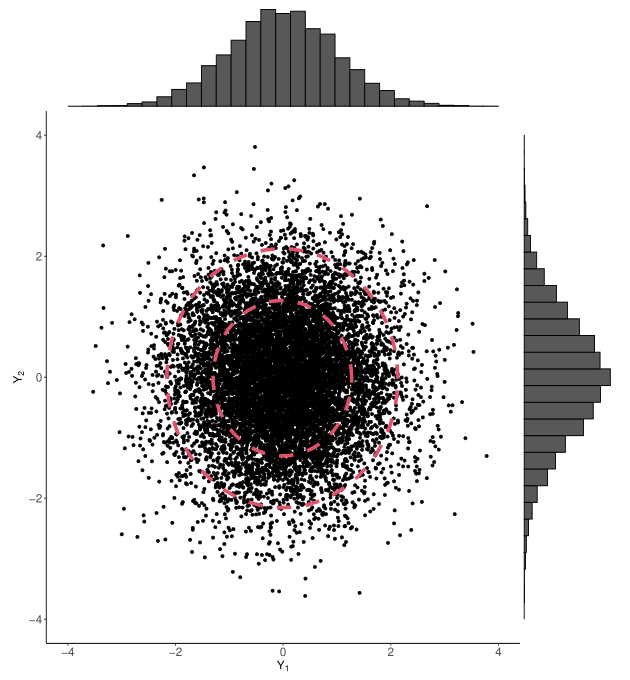
\includegraphics[width=0.65\textwidth]{images/Gaussiane/VettoreBivariatoIndipendenza.png}
    \caption{Nube di punti generata da una distribuzione gaussiana bivariata con componenti incorrelate \cite{wilkinson_introduction_2020}.}
    \label{correlazione1}
\end{figure}


\newpage
Si noti che la nube di punti è centrata in zero come conseguenza della scelta di $\bm{\mu}$. È facile calcolare $\rho_{Y_1,Y_2}=0$ che garantisce l'incorrelazione delle componenti del vettore gaussiano. Questo risultato si intuisce dalla forma della nube: dato un punto nella nube, la conoscenza della sua coordinata $Y_1$ non dà alcuna informazione sulla sua coordinata $Y_2$.\\
Si consideri ora $\bm{\mu} = \begin{pmatrix}0\\0\end{pmatrix}$ e $\mathbf{\Sigma}=\begin{pmatrix}1&0.9\\0.9&1\end{pmatrix}$. Generando nuovamente una nube di punti si ottiene quanto mostrato in figura \ref{correlazione2}.\\

%%%%%%%%%IMMAGINE
\begin{figure}[h]
    \centering
    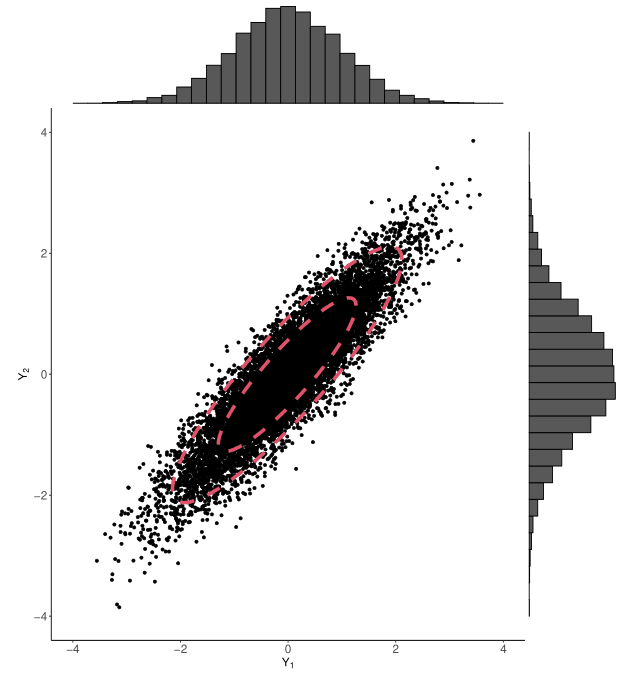
\includegraphics[width=0.7\textwidth]{images/Gaussiane/VettoreBivariatoIndipendenza2.png}
    \caption{Nube di punti generata da una distribuzione gaussiana bivariata con componenti correlate \cite{wilkinson_introduction_2020}.}
    \label{correlazione2}
\end{figure}

Dalla forma della nube è ora possibile notare la correlazione tra le componenti del vettore gaussiano. Dato un punto della nube, infatti, la prima delle due componenti dà un'idea approssimativa del valore della seconda componente (e viceversa): la nube, con una certa approssimazione, si addensa intorno ad una retta passante per l'origine.\\
La forma ellittica della nube è conseguenza del valore dell'indice di correlazione: $\rho_{Y_1,Y_2}=0.9$, cioè c'è una grande correlazione lineare tra le due componenti.\\

\newpage
Evidentemente la forma ellittica si accentua all'aumentare del valore dell'indice di correlazione, come è possibile notare dalla figura \ref{correlazione3}, nella quale $\mathbf{\Sigma}=\begin{pmatrix}1&0.99\\0.99&1\end{pmatrix}$ e dunque $\rho_{Y_1,Y_2}=0.99$.

%%%%%%%%%%%IMMAGINE
\begin{figure}[h]
    \centering
    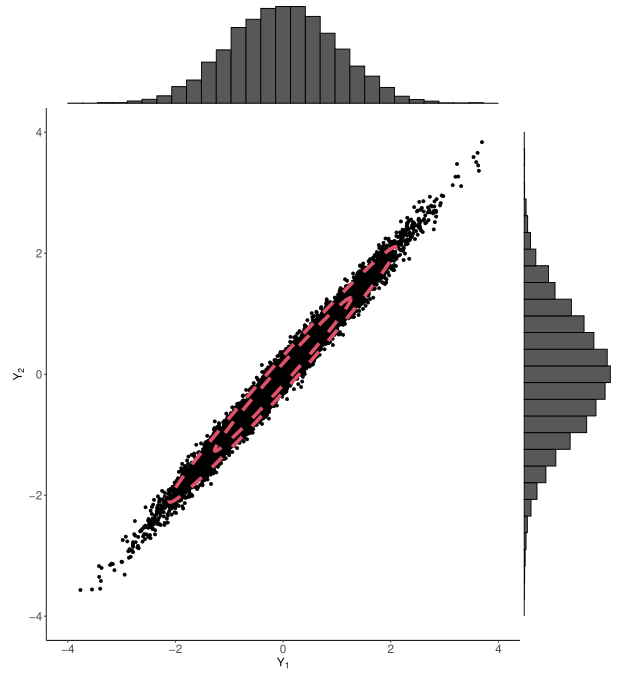
\includegraphics[width=0.7\textwidth]{images/Gaussiane/VettoreBivariatoIndipendenza3.png}
    \caption{Nube di punti generata da una distribuzione gaussiana bivariata con componenti fortemente correlate \cite{wilkinson_introduction_2020}.}
    \label{correlazione3}
\end{figure}

\newpage

Per poter generalizzare a più di due dimensioni il processo visivo di interpretazione della correlazione tra le componenti di un vettore gaussiano multivariato è necessario adottare una diversa strategia: per ogni campione (cioè per ogni vettore) generato dalla distribuzione gaussiana multivariata si traccia in un grafico il valore delle componenti collegando i rispettivi valori da un segmento.\\
In figura \ref{correlazione4} viene riportato l'esempio in due dimensioni con $\bm{\mu} = \begin{pmatrix}0\\0\end{pmatrix}$ e $\mathbf{\Sigma}=\begin{pmatrix}1&0.54\\0.54&0.3\end{pmatrix}$. Nel grafico a sinistra viene riportato l'approccio usato fino ad ora; nel grafico a destra per ogni punto del grafico a sinistra viene tracciato il valore della prima componente in corrispondenza dell'indice $1$ sulle ascisse e il valore della seconda componente in corrispondenza dell'indice $2$ sulle ascisse.


%%%%%%%%%%%IMMAGINE
\begin{figure}[h]
    \centering
    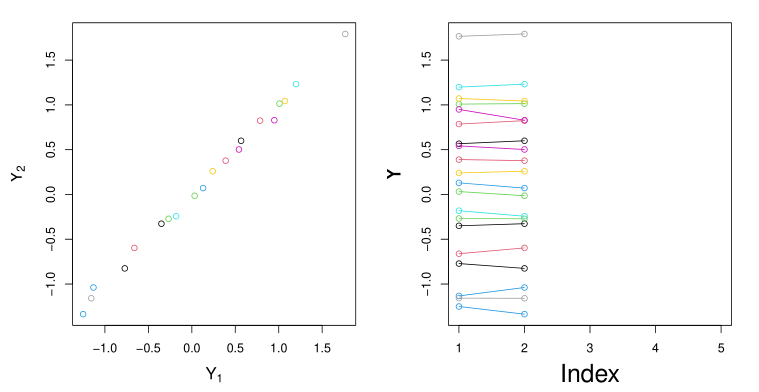
\includegraphics[width=\textwidth]{images/Gaussiane/CorrelazioneMultidimensionale.png}
    \caption{Due diversi approcci visivi alla correlazione di componenti di vettori gaussiani multivariati: $n=2$ \cite{wilkinson_introduction_2020}.}
    \label{correlazione4}
\end{figure}


\newpage 

Questo approccio permette di generalizzare a dimensioni $n>2$. Sia ora:
\[\bm{\mu}=\bm{0} \qquad\qquad \bm{\Sigma}=\begin{pmatrix}1&0.99&0.98&0.97&0.96\\0.99&1&0.99&0.98&0.97\\0.98&0.99&1&0.99&0.98\\0.97&0.98&0.99&1&0.99\\0.96&0.97&0.98&0.99&1 \end{pmatrix}
\]
dove le componenti sono fortemente correlate tra loro. Si ottiene quanto in figura \ref{correlazione5}.

%%%%%%%%%%%IMMAGINE
\begin{figure}[h]
    \centering
    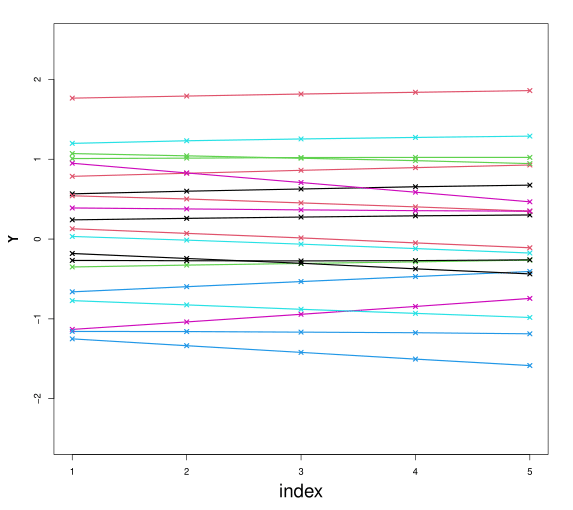
\includegraphics[width=0.7\textwidth]{images/Gaussiane/CorrelazioneMultidimensionale2.png}
    \caption{Visualizzazione tramite segmenti della correlazione di componenti di vettori gaussiani multivariati: $n=5$ \cite{wilkinson_introduction_2020}.}
    \label{correlazione5}
\end{figure}

Essendo in dimensione $n=5$, ogni campione generato dal vettore gaussiano ha cinque componenti, dunque quando un campione viene tracciato nel grafico ha cinque punti in corrispondenza degli indici 1, 2, 3, 4, 5.
\newpage

In questo caso, la forte correlazione tra le componenti del vettore gaussiano si riflette nel segmento che unisce i singoli punti di ogni campione, come mostrato in figura \ref{SegmentCorrelation}.

%%%%%%%%%%%IMMAGINE
\begin{figure}[h]
    \centering
    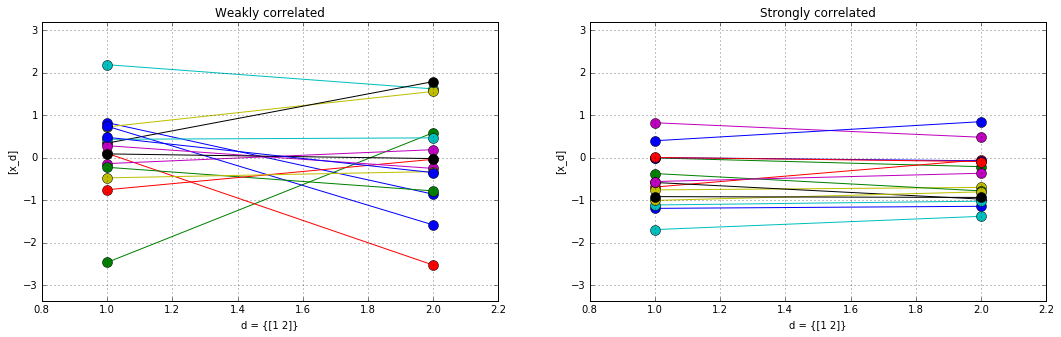
\includegraphics[width=1\textwidth]{images/Gaussiane/CorrelazioneUnidimensionale.png}
    \caption{Debole e forte correlazione delle componenti di vettori gaussiani multivariati visualizzata tramite segmenti \cite{damianou_gaussian_2016}.}
    \label{SegmentCorrelation}
\end{figure}

Nel caso $n=50$ (con vettore norma nullo ma omettendo la matrice di covarianza, che continua ad avere uno sulla diagonale e valori prossimi a uno nelle altre entrate), si ottiene quanto in figura \ref{correlazione6}.


%%%%%%%%%%%IMMAGINE
\begin{figure}[h]
    \centering
    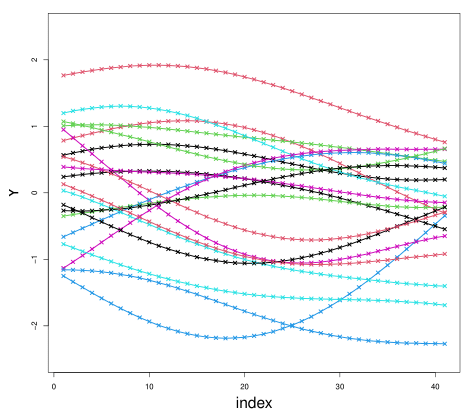
\includegraphics[width=0.7\textwidth]{images/Gaussiane/CorrelazioneMultidimensionale3.png}
    \caption{Visualizzazione tramite segmenti della correlazione di componenti di vettori gaussiani multivariati: $n=50$ \cite{wilkinson_introduction_2020}.}
    \label{correlazione6}
\end{figure}

Si noti quindi che all'aumentare di $n$ ciò che otteniamo inizia ad assomigliare a una funzione per ogni campione generato.\\
A partire da questa approccio è possibile interpretare i processi gaussiani come funzioni oppure come distribuzioni gaussiane multivariate infinito-dimensionali ($n=\infty$) con un indice continuo (introducendo una \textit{mean function} e una \textit{covariance function}). Questa interpretazione sarà chiarita nel prossimo capitolo.